\section{Distributed Concurrency Bugs}

One notorious type of software bugs is concurrency bugs. These timing-related
bugs manifest non-deterministically, and hence are extremely difficult to
detect, diagnose, and fix. A huge body of work exists in this space that
focuses on ``local'' concurrency (LC) bugs in single-machine multi-threaded
software, caused by incorrect interleaving of memory accesses.

Unfortunately, the reliability of datacenter distributed systems is severely
threatened by non-deterministic concurrency bugs as well, which we refer as
{\em distributed concurrency (DC) bugs}.  
% 
Distributed systems execute many complicated distributed protocols on
hundreds/thousands of machines with no common clocks. Moreover, cloud systems
run on large clusters of unreliable commodity machines, an environment that
produces a growing number and frequency of failures, including ``surprising''
failures \cite{Birman+09-CloudAgenda, Henry09-AmazonFUD}.  This combination
makes distributed systems prone to DC bugs caused by non-deterministic timing
of distributed events such as message arrivals, node crashes, node reboots, and
timeouts. It is common to see complex fault-induced DC bugs such as the one
in Figure \ref{fig-code-zk}.

%DC bugs cannot be directly tackled by LC bug techniques, and they cause fatal
%implications such as operation failures, downtimes, data loss and
%inconsistencies. 



\newcommand{\qbeg}{
\begin{quote}
%\begin{spacing}{0.9}
%\vminthree
}
\newcommand{\qend}{
%\vminten
%\end{spacing}
\end{quote}
}




\newcommand{\fev}[1]{\textcolor{Maroon}{\textit{#1}}}
\newcommand{\ev}[1]{\textcolor{gray}{\textbf{#1}}}


%\def \cbrk {\\}
\def \cbrk {}


\qbeg
{\small
{\bf ZooKeeper Bug \#335:}
\ev{(1)} Nodes A, B, C start with latest txid \#10 and elect
B as leader,
\ev{(2)} \fev{B crashes},
\ev{(3)} Leader election re-run; C becomes leader,
\ev{(4)} Client writes data; A and C commit new txid-value pair \{\#11:X\},
\ev{(5)} \fev{A crashes before} committing tx \#11,
\ev{(6)} C loses quorum,
\ev{(7)} \fev{C crashes},
\ev{(8)} \fev{A reboots} and \fev{B reboots},
\ev{(9)} A becomes leader,
\ev{(10)} Client updates data; A and B commit a new txid-value 
pair \{\#11:Y\},
\ev{(11)} \fev{C reboots after} A's new tx commit,
\ev{(12)} C synchronizes with A; C notifies A of \{\#11:X\},
\ev{(13)} A replies to C the ``diff'' starting 
with tx 12 (excluding tx \{\#11:Y\}!),
\ev{(14)} Violation: permanent data inconsistency as A and B
have \{\#11:Y\} and  C has \{\#11:X\}.
}
\qend



We look at 104 DC bugs from widely-deployed cloud-scale datacenter distributed
systems including Cassandra, Hadoop MapReduce, HBase, and ZooKeeper.
Statistically, Figure \ref{bars}a (\BFLT) shows that \pctFaultYes\ of DC bugs
must have at least one fault. In more detail, Figure \ref{bars}b-d (\BTO, \BCR,
\BRB) shows the percentage of issues that require timeouts, crashes and reboots
respectively, including how many instances of such faults must be there; the
rest is other faults such as disk errors (not shown).

\begin{figure}

\centerline{
\begin{tikzpicture}[font=\sffamily\footnotesize]
\begin{axis}[
xbar stacked,
y=0.8cm,
%width=5in,
width=\columnwidth,
%height=120pt,
xmin=0,
xmax=100,
bar width=12pt,  
%xmajorgrids=true,
%ylabel={Categorizations},
symbolic y coords={RB, CR, TO, FLT},
ytick=data,
yticklabels={{(d) RB, (c) CR, (b) TO, (a) FLT}},
every axis y label/.style={at={(ticklabel cs:0.5)},rotate=90,anchor=near ticklabel},
xticklabels={,,},
axis x line*=none,
x axis line style={opacity=0},
axis y line*=right
]
\addplot [fill=red!40] plot coordinates {(73.08,RB) (52.88,CR) (88.46,TO) (37.0,FLT)};
\addplot [fill=gray!40] plot coordinates {(20.19,RB) (34.62,CR) (11.54,TO) (63.0,FLT)};
\addplot [fill=pink!40] plot coordinates {(6.73,RB) (7.69,CR) (0,TO) (0,FLT)};
\addplot [fill=brown!40] plot coordinates {(0,RB) (4.81,CR) (0,TO) (0,FLT)};

\coordinate (rb0) at (36.54, -0.5);
\coordinate (rb1) at (83.175, -0.5);
\coordinate (rb2p) at (96.635, -0.5);
\coordinate (cr0) at (26.44, 99.5);
\coordinate (cr1) at (70.19, 99.5);
\coordinate (cr2) at (91.345, 99.5);
\coordinate (cr3p) at (97.595, 99.5);
\coordinate (toNo) at (44.23, 199.5);
\coordinate (toYes) at (94.23, 199.5);
\coordinate (fltNo) at (18.5, 299.5);
\coordinate (fltYes) at (68.5, 299.5);
\end{axis}

\node at (rb0) {0 (73\%)};
\node at (rb1) {1 (20\%)};
\node at (rb2p) {2+};
\node at (cr0) {0 (53\%)};
\node at (cr1) {1 (35\%)};
\node at (cr2) {2 (8\%)};
\node at (cr3p) {3+};
\node at (toNo) {No (88\%)};
\node at (toYes) {Yes (12\%)};
\node at (fltNo) {No (37\%)};
\node at (fltYes) {Yes (63\%)};

\end{tikzpicture}
%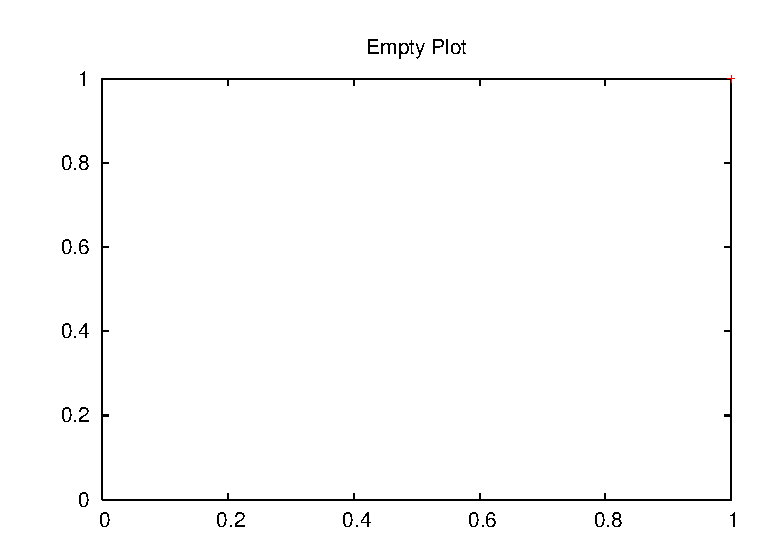
\includegraphics[width=1.8in]{F/empty.eps}
}
\vminten
\mycaption{bars}{Statistical overview of DC bugs}{}
% \vten

\end{figure}


%
\if 0
nodes (TSN), 
protocols (TSP), 
background (BR), 
triggering messages (TSM), 
local-message race (LM), 
timeout (TO),
crashes (CR),
reboots (RB),
errorMessage (EM),
reported (REP),  
implication (IMP),
control/data plane (CDP), 
\fi


\if 0
We can see that some DC bugs require complex conditions to manifest (\ie
multiple faults including crashes, reboots, timeouts, and other hardware
failures). We will discuss what is state of the art to find DC bugs in the next
section.
\fi

\subsection{Distributed Systems Model Checker (DMCK)}

In order to unearth DC bugs the question we have to answer is: ``{\em can we
exercise necessary conditions (\ie workloads and faults) and test different
event re-ordering to hit the bugs?}''. This is the job of distributed system
model checkers (dmck), which are gaining popularity recently
\cite{Guo+11-Demeter, Killian+07-LifeDeathMaceMC, Simsa+10-Dbug,
Yang+09-Modist}. Dmck works by intercepting distributed events and permuting
their ordering, and hereby pushing the target system into corner-case situations
and unearthing hard-to-find bugs. However, the more events included, the more
scalability issues will arise due to state-space explosion.




\begin{figure}[t]

\centerline{
%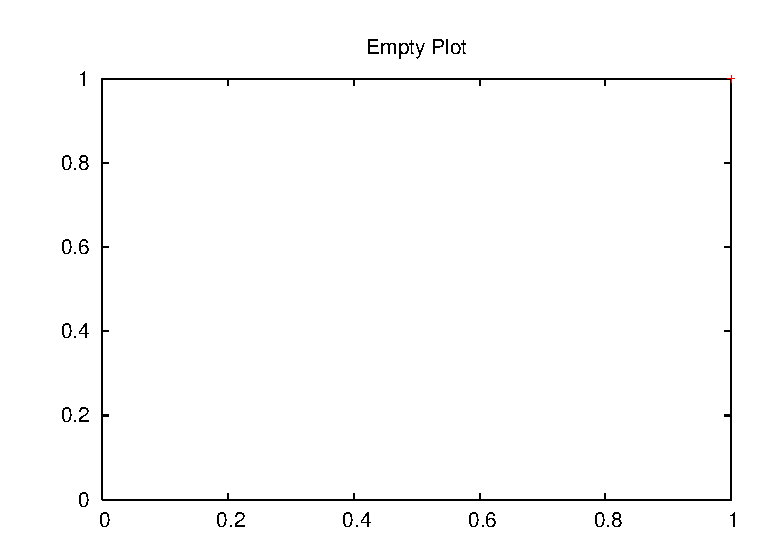
\includegraphics[height=1in]{F/empty.eps}
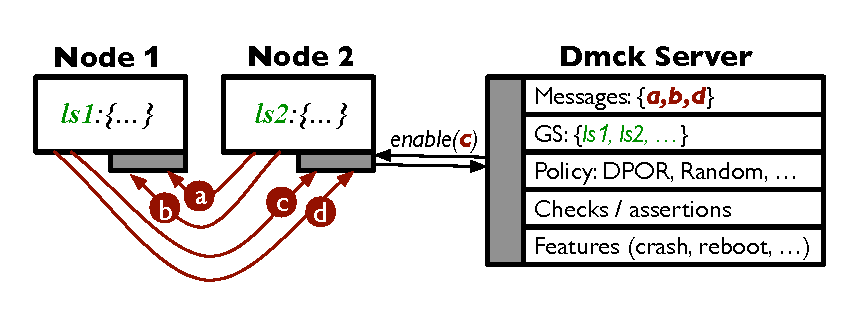
\includegraphics[height=2in]{F/dmck/dmck.eps}
}
\vminfive
\mycaption[Distributed System Model Checker]{fig-dmck}{DMCK}{The figure illustrates a typical framework
of a distributed system model checker (dmck).
}
%\vminten
\end{figure}

\if 0
The figure shows a dmck server model checking
a target distributed system containing two nodes.  
Communications in the target system are interposed 
\fi



The last seven years have seen a rise of software model checker that checks
distributed systems directly at the implementation level.  Figure~\ref{fig-dmck}
illustrates a dmck integration to a target distributed system, a simple
representation of existing dmck frameworks~\cite{Guo+11-Demeter,
Killian+07-LifeDeathMaceMC, Simsa+10-Dbug, Yang+09-Modist}.  The dmck inserts an
interposition layer in each node of the target system with the purpose of
controlling all important events (\eg, network messages, timeouts) and
preventing the target system to process the events until the dmck enables them.
A main dmck mechanism is the permutation of events; the goal is to push the
target system into all possible ordering scenarios.  For example, the dmck can
enforce \ts{abcd} ordering in one execution, \ts{bcad} in another, and so on.

\subsection{State-of-the-Art DMCKs}

\modist~\cite{Yang+09-Modist} is arguably one of the most powerful
dmcks that comes with systematic reduction policies.  \modist\ has been
integrated to real systems due to its exploration
scalability.  At the heart of \modist\ is {\em dynamic partial order
  reduction (DPOR)}~\cite{Flanagan+05-Dpor} which exploits the {\em
  independence} of events to reduce the state explosion.  Independent
events mean that it does not matter in what order the system execute
the events, as their different orderings are considered equivalent.

To illustrate how \modist\ adopts DPOR, let's use the example in
Figure~\ref{fig-dmck}, which shows four concurrent 
outstanding messages \ts{abcd}
(\ma\ and \mb\ for \none, \mc\ and \md\ for \ntwo).  A brute-force
approach will try all possible combinations (\ts{abcd}, \ts{abdc},
\ts{acbd}, \ts{acdb}, \ts{cabd}, and so on), for a total of 4!
executions.
% dpor
Fortunately, the notion of event independence can be mapped to
distributed system properties.  For example, \modist\ specifies this
reduction policy: a message to be processed by a given node is
independent of other concurrent messages destined to other nodes
(based on vector clocks).  Applying this policy to the example in
Figure~\ref{fig-dmck} implies that \ma\ and \mb\ are
dependent\footnote[1]{In model checking, ``dependent'' events mean
  that they must be re-ordered.  ``Dependent'' does not mean
  ``causally dependent''.}  but they are independent of \mc\ and
\md\ (and vice versa).  Since only dependent events need to be
reordered, this reduction policy leads to only 4 executions
(\ma\mb-\mc\md, \ma\mb-\md\mc, \mb\ma-\mc\md, \mb\ma-\md\mc), giving a
6x speed-up (4!/4).

Although \modist's speed-up is significant, we find that one 
scalability limitation of its DPOR application is within its {\em
  black-box} approach; it only exploits general properties of
distributed systems to define message independence.  It does not
exploit any semantic information from the target system to define more
independent events.  

% demeter
Dynamic interface reduction (DIR)~\cite{Guo+11-Demeter} is the next
advancement to \modist.  This work suggests that a complete dmck must
re-order not only messages (global events) but also thread
interleavings (local events).  The reduction intuition behind DIR is
that different thread interleavings often lead to the same global
events (\eg, a node sends the same messages regardless of how threads are
interleaved in that node).  DIR records local exploration and replays
future incoming messages without the need for global exploration.
In our work, SAMC focuses only on global exploration (message and fault
re-orderings).  We believe DIR is orthogonal to SAMC, similar to the
way DIR is orthogonal to \modist.

% besides (quick take)
\modist\ and DIR are examples of dmcks that employ advanced systematic
reduction policies.  LMC~\cite{Guerraoui+11-McNoNetwork} is similar to
DIR; it also decouples local and global exploration.
dBug~\cite{Simsa+10-Dbug} applies DPOR similarly to \modist.  There are
other dmcks such as \macemc~\cite{Killian+07-LifeDeathMaceMC} and
CrystalBall~\cite{Yabandeh+09-CrystalBall} that use basic exploration
methods such as depth first (DFS), weight-based,
and random searches.

% symmetry
Other than the aforementioned methods, {\em symmetry} is another
foundational reduction policy~\cite{Emerson+97-PorAndSym,
  Prasad+00-SymBasedMc}.  Symmetry-based methods exploit the
architectural symmetry present in the target system.  For example, in
a ring of nodes, one can rotate the ring without affecting
the behavior of the system.  Symmetry is powerful, but
we find no existing dmcks that adopt symmetry.

% multiple failures
Besides dmcks, there exists sophisticated testing frameworks for
distributed systems (\eg, \fate~\cite{Gunawi+11-FateDestini},
\prefail~\cite{Joshi+11-PreFail},
\setsudo~\cite{Joshi+13-SetsudoTesting}, OpenStack
fault-injector~\cite{Ju+13-FaultResOpenStack}). This set of work
emphasizes the importance of multiple faults, but their major
limitation is that they are not a dmck.  That is, they cannot
systematically control and permute non-deterministic choices such as
message and fault reorderings.
